    \documentclass[11pt,
        usenames, % allows access to some tikz colors
        dvipsnames % more colors: https://en.wikibooks.org/wiki/LaTeX/Colors
    ]{article}
    \usepackage{
        amsmath,
        amssymb,
        fouriernc, % fourier font w/ new century book
        fancyhdr, % page styling
        lastpage, % footer fanciness
        hyperref, % various links
        setspace, % line spacing
        amsthm, % newtheorem and proof environment
        mathtools, % \Aboxed for boxing inside aligns, among others
        float, % Allow [H] figure env alignment
        enumerate, % Allow custom enumerate numbering
        graphicx, % allow includegraphics with more filetypes
        wasysym, % \smiley!
        upgreek, % \upmu for \mum macro
        listings, % writing TrueType fonts and including code prettily
        tikz, % drawing things
        booktabs, % \bottomrule instead of hline apparently
        cancel % can cancel things out!
    }
    \usepackage[margin=0.8in]{geometry} % page geometry
    \usepackage[
        labelfont=bf, % caption names are labeled in bold
        font=scriptsize % smaller font for captions
    ]{caption}
    \usepackage[font=scriptsize]{subcaption} % subfigures
    \usepackage[numbers]{natbib}

    \newcommand*{\scinot}[2]{#1\times10^{#2}}
    \newcommand*{\dotp}[2]{\left<#1\,\middle|\,#2\right>}
    \newcommand*{\rd}[2]{\frac{\mathrm{d}#1}{\mathrm{d}#2}}
    \newcommand*{\pd}[2]{\frac{\partial#1}{\partial#2}}
    \newcommand*{\rtd}[2]{\frac{\mathrm{d}^2#1}{\mathrm{d}#2^2}}
    \newcommand*{\ptd}[2]{\frac{\partial^2 #1}{\partial#2^2}}
    \newcommand*{\md}[2]{\frac{\mathrm{D}#1}{\mathrm{D}#2}}
    \newcommand*{\pvec}[1]{\vec{#1}^{\,\prime}}
    \newcommand*{\svec}[1]{\vec{#1}\;\!}
    \newcommand*{\bm}[1]{\boldsymbol{\mathbf{#1}}}
    \newcommand*{\ang}[0]{\;\text{\AA}}
    \newcommand*{\mum}[0]{\;\upmu \mathrm{m}}
    \newcommand*{\at}[1]{\left.#1\right|}

    \newtheorem{theorem}{Theorem}[section]

    \let\Re\undefined
    \let\Im\undefined
    \DeclareMathOperator{\Res}{Res}
    \DeclareMathOperator{\Re}{Re}
    \DeclareMathOperator{\Im}{Im}
    \DeclareMathOperator{\Log}{Log}
    \DeclareMathOperator{\Arg}{Arg}
    \DeclareMathOperator{\Tr}{Tr}
    \DeclareMathOperator{\E}{E}
    \DeclareMathOperator{\Var}{Var}
    \DeclareMathOperator*{\argmin}{argmin}
    \DeclareMathOperator*{\argmax}{argmax}
    \DeclareMathOperator{\sgn}{sgn}
    \DeclareMathOperator{\diag}{diag\;}

    \DeclarePairedDelimiter\bra{\langle}{\rvert}
    \DeclarePairedDelimiter\ket{\lvert}{\rangle}
    \DeclarePairedDelimiter\abs{\lvert}{\rvert}
    \DeclarePairedDelimiter\ev{\langle}{\rangle}
    \DeclarePairedDelimiter\p{\lparen}{\rparen}
    \DeclarePairedDelimiter\s{\lbrack}{\rbrack}
    \DeclarePairedDelimiter\z{\lbrace}{\rbrace}

    % \everymath{\displaystyle} % biggify limits of inline sums and integrals
    \tikzstyle{circ} % usage: \node[circ, placement] (label) {text};
        = [draw, circle, fill=white, node distance=3cm, minimum height=2em]
    \definecolor{commentgreen}{rgb}{0,0.6,0}
    \lstset{
        basicstyle=\ttfamily\footnotesize,
        frame=single,
        numbers=left,
        showstringspaces=false,
        keywordstyle=\color{blue},
        stringstyle=\color{purple},
        commentstyle=\color{commentgreen},
        morecomment=[l][\color{magenta}]{\#}
    }

\begin{document}

\def\Snospace~{\S{}} % hack to remove the space left after autorefs
\renewcommand*{\sectionautorefname}{\Snospace}
\renewcommand*{\appendixautorefname}{\Snospace}
\renewcommand*{\figureautorefname}{Fig.}
\renewcommand*{\equationautorefname}{Eq.}
\renewcommand*{\tableautorefname}{Tab.}

\singlespacing

\pagestyle{fancy}
% \rfoot{Yubo Su}
\rhead{}
\cfoot{\thepage/\pageref{LastPage}}

\title{Q Exam Written Report}
\author{Yubo Su\\
Adviser: Dong Lai}

\maketitle

\section{Introduction: White Dwarf Binaries}

White Dwarfs (WDs) are commonly found in binaries in which two objects orbit
their center of mass under mutual gravitational attraction. The companion object
ranges from another WD to a supermassive BH (SMBH). Understanding the evolution
of such systems is important to astrophysics. WD-WD binaries are most important
for being thought to generate Type Ia supernovae which have been used as a
``standard candle'' to probe the expansion rate of the
universe\cite{darkEnergy}. WD-BH systems are also interesting subjects of study.
Recent works indicate that as WDs plunge close to BHs, they will produce
observable flares induced by gravitational tidal forces\cite{flares}. A WD
orbiting a SMBH would also produce gravitational waves that are expected to be
detected by the space-based \emph{Laser Interferometer Space Antenna (LISA)}
when deployed\cite{lisa}. Gravitational wave astronomy is an increasingly
exciting field as the \emph{Laser Interferometer Gravitational-Wave Observatory
(LIGO)} continues to make progress since its first detection in late 2015. As
gravitational wave astronomy relies on accurate predictions of the expected
signals, it is important to build as accurate models as possible before
observation runs begin.

\subsection{Tidal Dissipation}

The excitation of \emph{internal gravity waves} (IGW) in the WD by the tidal
forces of the companion is an effect exhibited in the aforementioned systems.
IGWs, not to be confused with the gravitational waves above, are internal
displacements in the WD fluid that oscillate and propagate due to a restoring
buoyancy force. Previous work\citep{fullerI} indicates that IGWs can be excited
in WD binaries that propagate outwards and grow exponentially due to density
rarefaction, reaching nonlinear amplitudes well before the WD boundary. These
waves are then expected to break and dissipate via nonlinear processes.

Previous work predicts that this dissipation mechanism can generate
significantly more energy than thermal radiation from the WD surface alone and
are thus a significant contribution to the WD energy budget\cite{fullerII}. The
exact radial dissipation profile is of interest since it both is sensitive to WD
properties and can produce vastly different observable outcomes. One proposed
outcome is a \emph{tidal nova}, in which heating in the WD's degenerate hydrogen
layer is sufficient to trigger runaway nuclear fusion and an observable surface
explosion\cite{tidal_novae}. Understanding whether such phenomena occur requires
understanding how energy and angular momentum are redistributed internally
inside the WD\@.

Internal gravity wave breaking is a nonlinear hydrodynamic phenomenon. Such
phenomena are known to require numerical simulation to study in detail.

\section{Work Accomplished: Theory and Numerics}

To begin our numerical study of IGW breaking, we first considered 2D IGW
breaking in a plane-parallel, uniformly stratified, incompressible atmosphere.
Even in this reduced problem, we encountered numerous difficulties and efforts
to surmount them are ongoing. Thus the subsequent two sections on the theory and
numerics of IGW breaking largely focus on the toy problem with only brief
references to extensions to the full 3D, compressible problem we wish to
eventually study.

\subsection{IGW Theory}

\subsubsection{IGW System and Linear Theory}

We briefly recap the studied IGW system in detail and its solution in linear
theory. An incompressible 2D hydrodynamical system can be described by just four
Eulerian dynamical variables $\rho, P, u_x, u_z$, the density, pressure and $x,
z$ components of Eulerian velocity respectively, each of which is a function of
$x, z, t$. We notate $\rho = \rho_0 + \rho_1$ where $\rho_0$ is the background
density satisfying hydrostatic equilibrium in the absence of any IGW and
$\rho_1$ is the deviation that represents the IGW flow, and likewise for the
remaining variables. In the linear theory, we assume $\rho_1 \ll \rho_0, P_1 \ll
P_0$, and to further simplify the problem we take $u_{0x} = u_{0z} = 0$. The
resulting system of equations describing IGW propagation are:
\begin{subequations}\label{se:igw_lin}
    \begin{align}
        \vec{\nabla} \cdot \vec{u}_1 &= 0,\\
        \rd{\rho_1}{t} + u_{1z}\pd{\rho_0}{z} &= 0,\\
        \rd{\vec{u}_1}{t} + \frac{\vec{\nabla}P_1}{\rho_0}
            - \rho_1 \frac{\vec{\nabla}P_0}{\rho_0^2} &= 0.
    \end{align}
\end{subequations}
In the linearized system, $\rd{}{t} = \pd{}{t} + \vec{u} \cdot \vec{\nabla}
\approx \pd{}{t}$. Uniform stratification takes the form $-\pd{\ln \rho_0}{z} =
-\pd{\ln P_0}{z} = H$ where $H$ is some characteristic scale height, then it can
be shown the IGW solution takes on form
\begin{align}
    u_{1z}(x, z, t) &= Ae^{z/2H}e^{i\p*{k_xx + k_zz - \omega(k_x, k_z) t}},
        \label{eq:plane}\\
    \omega(k_x, k_z) &= \frac{Nk_x}{\sqrt{k_x^2 + k_z^2 + \frac{1}{4H^2}}},
\end{align}
where $N^2 = \frac{g}{H}$ the Brunt-V\"ais\"al\"a frequency is constant. Note
the $u_{1z} \propto e^{z/2H}$ growth induced by the density stratification, and
so we expect nonlinear effects to become important as $Ae^{z/2H} \sim 1$.

\subsubsection{Nonlinear IGW Theory}

The leading-order nonlinearities in \autoref{se:igw_lin} causing the plane wave
solution \autoref{eq:plane} to break down are thoroughly studied in atmospheric
sciences e.g.\cite{Sutherland1}\cite{Sutherland2}, though a verdict on the exact
breaking phenomenon is still unclear. The primary two mechanisms considered by
the community are:
\begin{description}
    \item[Modulational Instability] By arguments similar to those underlying
        Stokes Flow (the mean motion of particles in a plane wave flow), it can
        be shown that the plane wave solution \autoref{eq:plane} induces a mean
        flow $\mathcal{O}(A^2)$. Since, in the incompressible system, $\vec{k}
        \cdot \vec{u} = 0$ (where $\vec{k} = k_x\hat{x} + k_z\hat{z}$ is the
        wave vector), many of the advective terms $\vec{u} \cdot \vec{\nabla}$
        vanish to second order $\vec{u}_1 \cdot \vec{\nabla}\vec{u}_1 = 0$, and
        so the first nonlinear term to appear must be the interaction of the
        plane wave with its own induced mean flow.

        With some algebraic manipulations, \autoref{se:igw_lin} can be recast in
        the form of a nonlinear Schr\"odinger Equation, whose form is $iA_t =
        \alpha A_{xx} + \beta \abs*{A}^2A$. $A$ happens here to be the complex
        amplitude of the Eulerian displacement, and $\abs*{A}^2$ is the mean
        flow term.

        The weakly nonlinear Schr\"odinger equation can be examined for
        \emph{modulational instability} by considering the evolution of modes
        near the propagating plane wave, i.e.\ a wave train centered on
        $\vec{k}_0$. A brief derivation of the criterion is provided
        in~\cite{Whitham} and applied in~\cite{Sutherland1}. The calculations
        show that for certain values of $\vec{k}$, the wave propagates with a
        weakly split group velocity that acts to reduce the amplitude and delay
        breaking, while for other values the group velocity is complex and
        exhibits breaking at lower amplitudes. An exmaple of a modulationally
        unstable Gaussian wavepacket is shown in \autoref{fig:modinstab}.
        \begin{figure}[t]
            \centering
            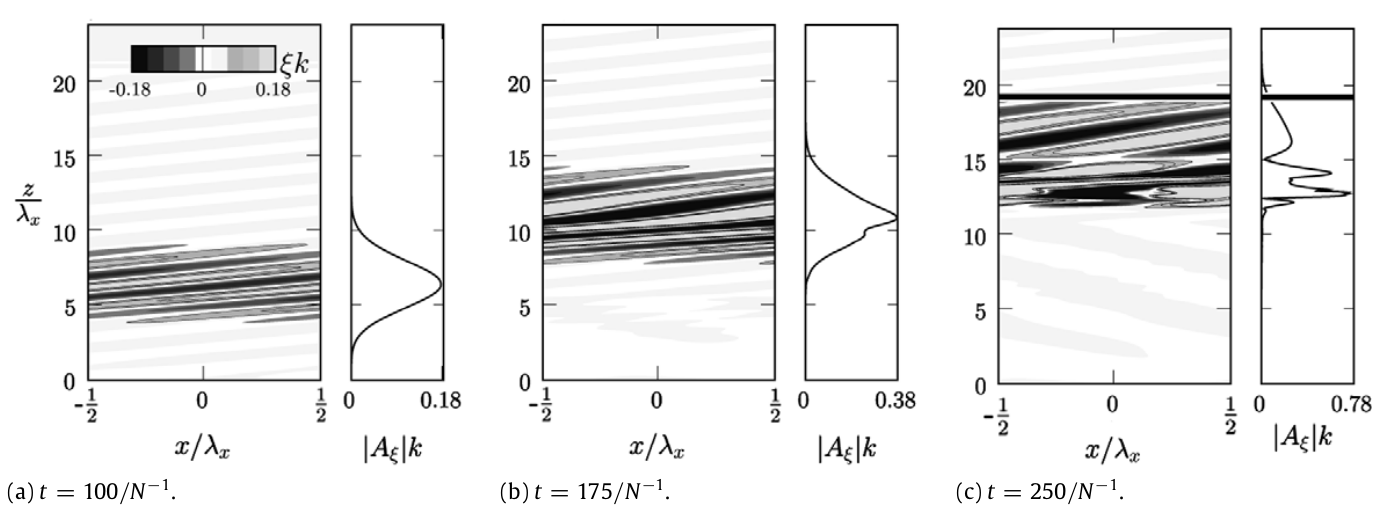
\includegraphics[width=\textwidth]{figs/sutherland_modinstab.png}
            \caption{Modulationally unstable wavepacket breaking before the
            height predicted by linear theory (thick black
            line).}\label{fig:modinstab}
        \end{figure}

    \item[Parametric Subharmonic Instability] If a triad of modes with
        wavevectors $\vec{k}_1, \vec{k}_2, \vec{k}_3$ satisfies the triad
        resonance condition
        \begin{align}
            \vec{k}_1 &= \vec{k}_2 + \vec{k}_3 &
            \omega(\vec{k}_1) &= \omega(\vec{k}_2) + \omega(\vec{k}_3),
            \label{eq:triad}
        \end{align}
        then it is possible in the nonlinear advective term $\vec{u} \cdot
        \vec{\nabla}$ for two modes to have a frequency component that drives
        the third. A careful albeit tedious derivation for the growth rate of
        two infinitesimal modes in the presence of a third mode such that the
        three satisfy \autoref{eq:triad} is given in~\cite{psi}. Further Floquet
        analysis, as done in~\cite{DrazinFloquet}, illustrates that this
        produces cascades to integer multiples of the plane wave wavevector and
        fractions of the temporal frequency.

        It bears noting that, as this is a parametric resonance, the growth of
        the subharmonics grows exponentially from a nonzero initial value. An
        example of the development of these higher modes is given in
        \autoref{fig:igw_psi}.
        \begin{figure}[t]
            \centering
            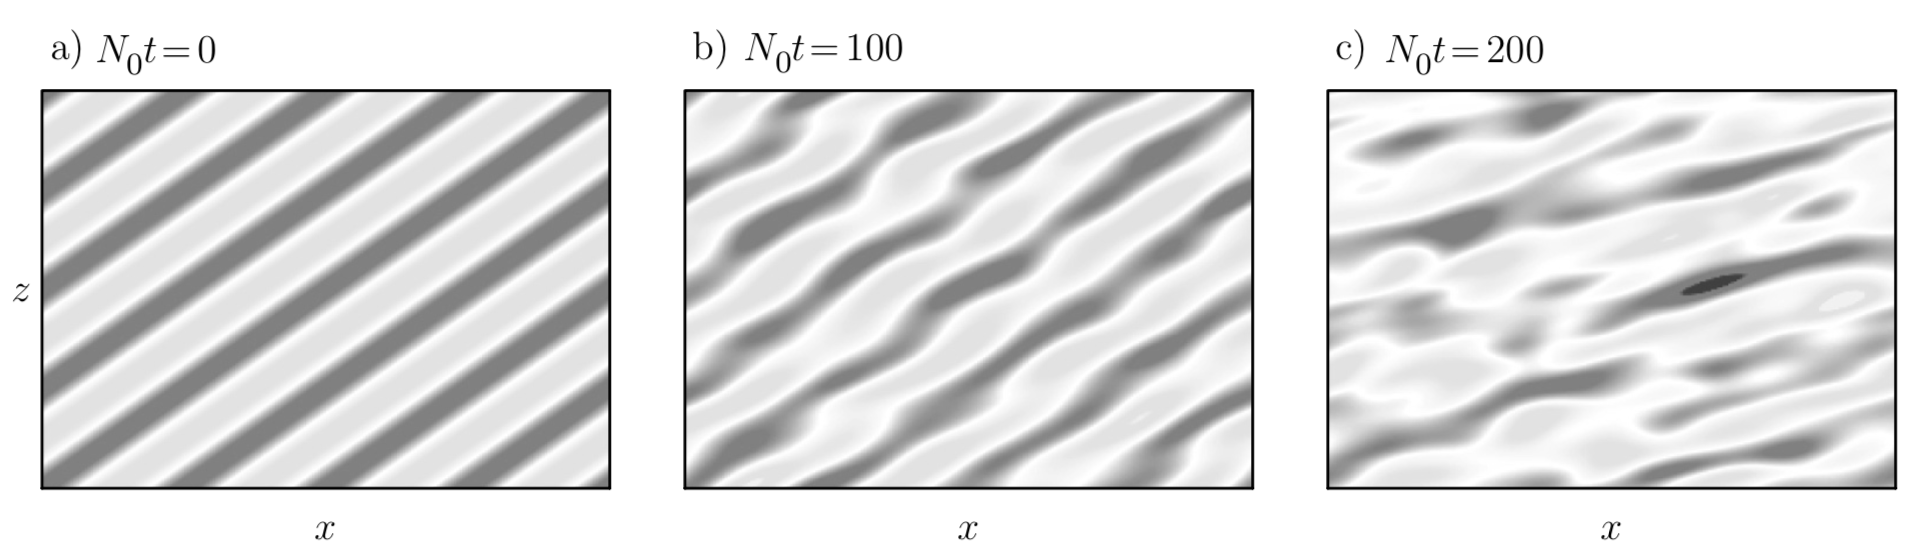
\includegraphics[width=0.8\textwidth]{figs/igw_psi.png}
            \caption{Breakdown of plane wave via parametric subharmonic
            instability. Doubly periodic boundary conditions, courtesy
            of~\cite{SutherlandBook}.}\label{fig:igw_psi}
        \end{figure}
\end{description}

While a thorough understanding of the nonlinear theory is not strictly
necessary to run simulations, it is important to be able to identify whether
deviations from the linear solution in simulations are numerical artifacts or
real physical effects.

\subsection{Numerical Simulations}

\subsubsection{Choice of Software}

For numerical simulations we use the spectral PDE solver
\lstinline{Dedalus}\cite{dedalus}. A number of concerns motivated our choice of
software:
\begin{itemize}
    \item Though we expect the problem to develop fine scale structure at later
        times, no shocks develop. Spectral methods exhibit exponential
        convergence when dynamical variables vary smoothly\cite{NR}, and so we
        are able to capture better numerical precision for the same
        computational cost.

    \item As the key focus of our study is how energy cascades into smaller
        length scales but we have limited spatial resolution, we must introduce
        some nonphysical regularization at small length scales to prevent them
        from accumulating energy. This usually comes in the form of viscosity,
        so having precise control over the viscosity is necessary to understand
        the regime of validity of our results. Spectral methods have no
        numerical viscosity\cite{NR} and so allow for much more precise control
        over regularization.

    \item \lstinline{Dedalus} is an exceptionally easy to use code and remains
        under active development. It also comes parallelized and has been
        extended to 3D geometries as well (although still in development).
\end{itemize}
Note however that \lstinline{Dedalus}, being a fully spectral solver, does not
support numerical techniques such as adaptive mesh refinement and so must use a
uniform resolution throughout the simulation domain. It is thus prudent to
choose a simulation subject that maximizes usage of the domain with interesting
behavior.

\subsubsection{Setup}

Note that the objective only requires simulating IGWs near the end of their
propagation, after an infinitesimal displacement has already grown to
near-nonlinear amplitudes. Focusing on the end of their evolution is a
tremendous computational savings both in temporal evolution and spatial
resolution as discussed above.

We discuss the simulation setup and its various considerations below:
\begin{description}
    \item[Domain] We choose a 2D domain with periodic boundary conditions in the
        $x$ direction and aperiodic boundary conditions in the $z$ direction to
        permit density stratification. In conjunction with the damping zones
        below, this mimics a 2D infinite plane geometry. The choice of spectral
        basis functions is then Fourier in the $x$ and Chebyshev in the $z$.

        We want a $z$ domain of a many scale heights to induce growth to
        nonlinear amplitudes, so we use $z \in [0, 10H]$. To use a similarly
        sized domain, we use $x \in [0, 4H]$.

        We are able to use $1024$ Chebyshev modes and $256$ Fourier modes
        (memory and computation resource limited), meaning we can resolve length
        scales $\sim H/100$, plenty for our target $k_z = \frac{20}{H}$.

    \item[Damping Zones] In order to mimic an unbounded domain in the $z$, we
        must ensure that the boundaries do not produce reflections. Such
        radiative boundary conditions (also outgoing/Sommerfield/absorbing
        boundary conditions) can only be approximate when applied to many
        $\vec{k}$ incoming waves\cite{RadBC}\cite{Wagatha1983}.

        Instead, we implement \emph{damping zones} modeled after those used
        in~\cite{LecoanetDamp}. We introduce a field $\Gamma(z)$ such that
        $\pd{}{t} \to \pd{}{t} + \Gamma(z)$, so that dynamical variables
        dissipate where $\Gamma$ is nonzero. Choosing then $\Gamma$ to vanish
        everywhere but near the boundaries suppresses reflection. In order to
        ensure $\Gamma(z)$ has an exponentially convergent spectral
        representation, we must choose smooth $\Gamma(z)$, and a traditional
        choice is (let $z \in [0, L_z]$ be the simulation domain)
        \begin{equation}
            \Gamma(z) = \frac{\Gamma_0}{2}\s*{
                2 + \tanh \gamma\frac{z - z_t}{L_z - z_t} +
                    \tanh \gamma\frac{z_b - z}{z_b}
            }.
        \end{equation}
        This function is approximately zero $z \in [z_b, z_t]$ and approximately
        $1$ in the damping zones. Furthermore, its steepness can be tuned via
        the parameter $\gamma$ (it cannot be so steep as to run up against
        spatial resolution, however), and the damping timescale can be tuned by
        $\Gamma_0$.

        In our simulation, $z_b = 0.07L_z, z_t = 0.93L_z, \gamma = 3$ and we
        choose $\Gamma_0 = N$ such that, in the damping zone oscillations damp
        on the timescale of $N^{-1}$.

    \item[Forcing] Since we only wish to model the later stages of IGW
        evolution, we need only excite an IGW in the linear regime with any
        mechanism rather than specifically the tidal mechanism describe in the
        introduction.

        Because Chebyshev polynomials (which satisfy $T_n(x) = \cos
        \p*{n \arccos x}$) have spacing between zeros scaling as $n^{-1}$ on the
        interior of the domain but cluster as $n^{-2}$ near the edge of the
        domain, the effective Courant-Friedrichs-Levy condition is much stricter
        when spectral features exist near the edge of the
        domain\cite{GottliebCFL}.

        Instead, we again follow~\cite{LecoanetDamp} in using a volumetric
        forcing term to generate a plane wave IGW\@. We choose a forcing profile
        of form
        \begin{equation}
            F(x, z, t) = F_0
                e^{-\frac{\p*{z - z_0}^2}{2\sigma^2}}e^{i(k_xx - \omega_0 t)}.
        \end{equation}
        If $\sigma$ is chosen to be sufficiently small, then $F(x, z, t)$ will
        have a reasonably large component along the $k_z$ wavevector satisfying
        $\omega(k_x, k_z) = \omega_0$ where $\omega(k_x, k_z)$ is the IGW
        dispersion relation. Thus we are able to drive on resonance and generate
        IGW propagating in both directions from $z_0$. Lastly, if we choose
        $z_0$ near the bottom of the domain, the upward propagating wave is
        exactly what we wish to study and the downward propagating wave is
        damped by the damping zone.

        Since our equations of motion require the velocity to be
        divergence-free, we instead attach the driving term to the \emph{density
        equation}. While this is ill-justifiable physically, corresponding to
        violating the conservation of mass periodically, it suffices for the
        application at hand. Thus, we use continuity equation
        \begin{equation}
            \rd{\rho_1}{t} - \rho_0 \frac{u_{1z}}{H} + \Gamma(z) \rho_1
                = F_0 e^{-\frac{\p*{z - z_0}^2}{2\sigma^2}}
                    \cos(k_xx - \omega_0 t).
        \end{equation}

        It is not so hard to compute the excited $u_{1z}(z = z_0)$ for such a
        forcing profile: solving for a forcing $F(x, z, t) = F_0\delta\p*{z -
        z_0}e^{i(k_xx - \omega_0t)}$ is a simple matter of matching homogeneous
        solutions, then an approximation that the Gaussian excites
        a $e^{-k_z^2\sigma^2/2}$ smaller wave is a serviceable approximation.
        This gives
        \begin{equation}
            \abs*{u_{1z}(z = z_0)} = \frac{F_0\sqrt{2\pi}\sigma gk_x^2}{
                2\rho_0\p*{z = z_0}\omega^2 k_z}e^{-k_z^2\sigma^2/2}.
        \end{equation}

        In order for the above approximation to hold, $\sigma$ must be small, so
        that the forcing is broad in spatial frequencies. We choose $\sigma k_z
        = 1$. We also use $z_0 = 0.25L_z$, so $0.1L_z$ separated from the
        damping zone, and we choose $F_0$ depending on the $u_{1z}(z = z_0)$
        desired (often $0.01$).

    \item[Timestepping] The primary timestep that must be resolved for IGW is
        $N^{-1}$ the buoyancy timescale (in IGW, $k_x \ll k_z$ and so $\omega
        \ll N$), so we have been testing with timesteps $\Delta t = 0.02N^{-1}$.
        Other simulations use a variety of timesteps $\Delta t \in
        [0.0025N^{-1}, 0.08N^{-1}]$
        e.g.~\cite{LecoanetDamp},~\cite{Sutherland1}. Because Dedalus uses
        implicit timestepping for linear terms, an overly large timestep induces
        amplitude loss during propagation; the proper diagnostic for timestep
        size is ensuring $e^{z/2H}$ growth in the linear regime.

    \item[Viscosity] This is the current stage of our work and is not yet
        well-characterized. Viscosity serves to regularize the system and
        drain energy preferentially from high $k_z$ modes. In order to maintain
        exponential convergence, we need to ensure that any mode that excites
        modes beyond the scope of our spectral expansion must be viscously
        damped. Thus, our regularization should damp the upper half of spectral
        modes.

        There are two choices for implementing such viscous regularization that
        we are currently investigating:

        \begin{description}
            \item[Navier-Stokes Viscosity] This is the traditional Navier-Stokes
                viscosity, which modifies the momentum equation of
                \autoref{se:igw_lin} as
                \begin{equation}
                    \rd{\vec{u}_1}{t} + \frac{\vec{\nabla}P_1}{\rho_0}
                        + \frac{\rho_1\vec{g}}{\rho_0} + \Gamma \vec{u}_1
                        - \nu \nabla^2 \vec{u}_1 = 0.
                \end{equation}

                Using our (rather heuristic) argument that half of modes should
                be damped in the nonlinear regime $u_1 \sim \frac{\omega}{k_z}$
                then we need $\nu \sim \omega \p*{\frac{L_z}{\pi N_Z}}^2$ where
                $N_Z$ is the number of $z$ modes. Note that $k_x\ll k_z$ does
                not factor into the $\nu \nabla^2$ size calculation.

            \item[Hyperviscosity] Much more of a numerical trick,
                \emph{hyperviscosity} refers to a family of
                stronger-than-Navier-Stokes viscosities. The one we consider is
                reaching directly into the $k_z$ spectral coefficients and
                artificially decreasing those beyond $N_Z/2$. Conventionally,
                hyperviscosity sets these directly to zero but this seems to be
                too strong by our tests. Because results are still pending, the
                exact hyperviscosity procedure is yet to be determined.
        \end{description}

    \item[Gradual Forcing] One last trick that we are considering is to turn on
        the forcing term gradually; \autoref{fig:plots} shows many examples
        where ringing from turning the forcing term on immediately excites
        ringing that generates spurious nonlinear interactions. We choose to
        effect this by $F(t) \tanh 10\omega_0t$, so over the course of about
        twenty periods the forcing will reach full amplitude. Results are
        pending.
\end{description}

$N^{-1}$ is the unit of time and $H$ the unit of distance in our computations,
both of which are set to $1$. Some snapshots from our simulation can be seen in
\autoref{fig:plots}. Note the smooth
\begin{figure}[t]
    \centering
    \begin{subfigure}{0.47\textwidth}
        \centering
        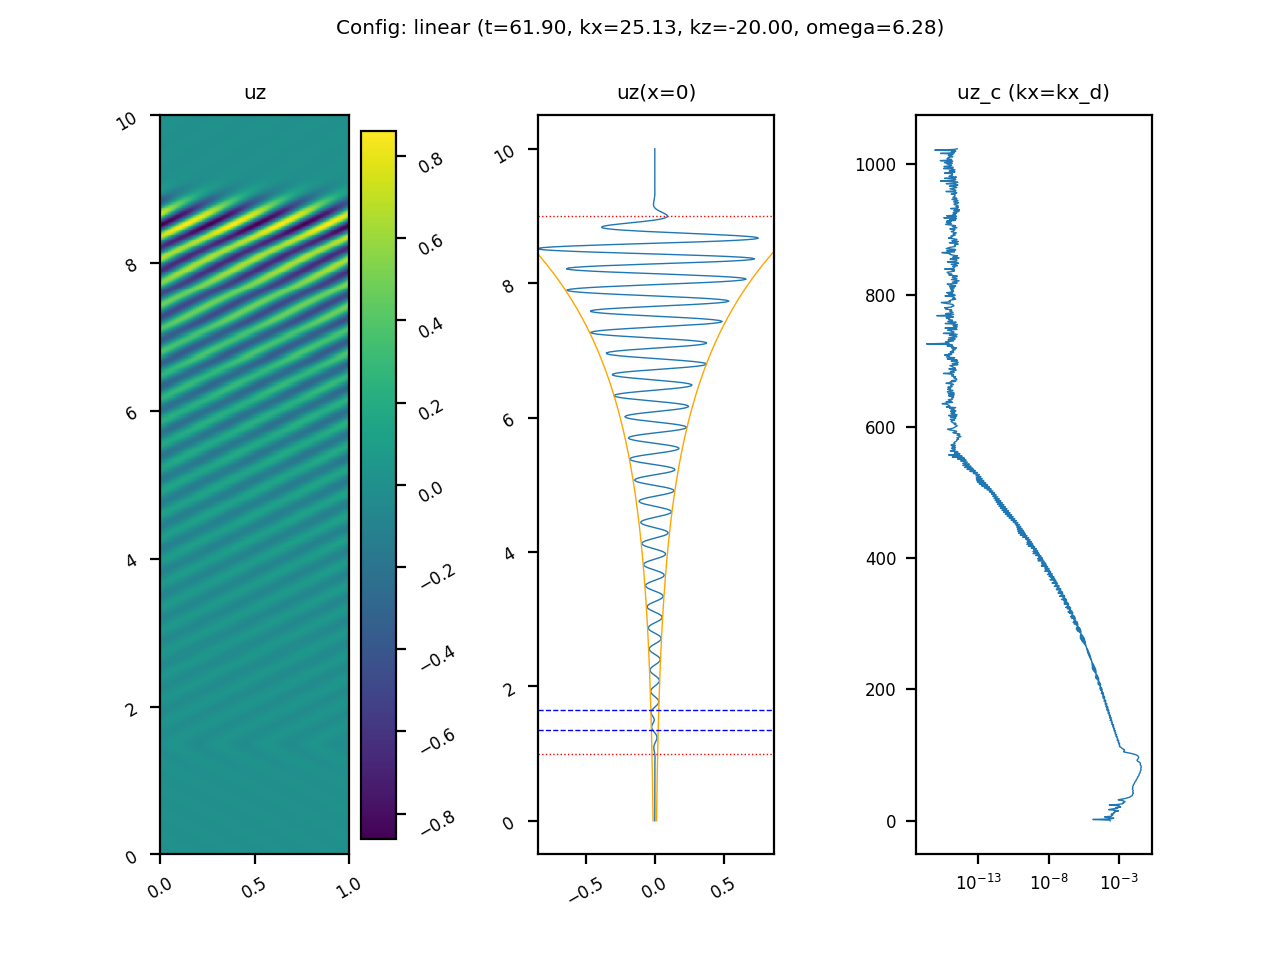
\includegraphics[width=\textwidth]{figs/linear.png}
        \caption{Linear simulation. Note the close agreement of the analytically
        predicted excitement amplitude and the actual waveform. The spectrum is
        broader than a pure Fourier spectrum due to the waveforms being
        sinusoidal and the basis being Chebyshev.}
    \end{subfigure}\hfill
    \begin{subfigure}{0.47\textwidth}
        \centering
        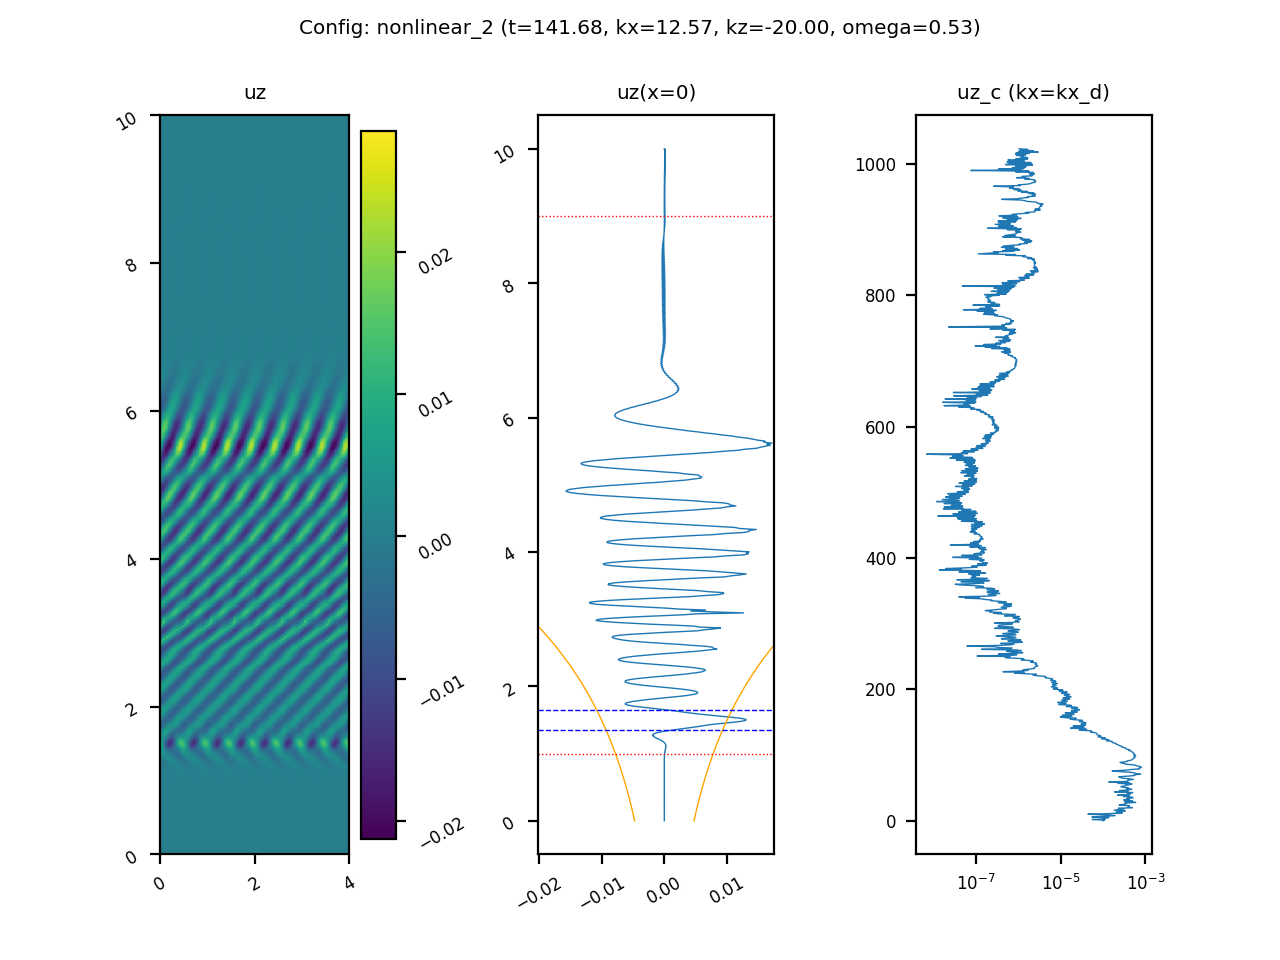
\includegraphics[width=\textwidth]{figs/nonlin_psi.png}
        \caption{Nonlinear simulation without regularization. The mismatch of
        the analytical envelope is not significant. Note the significant
        amplitude in higher Chebyshev modes. The simulation breaks soon after
        this point, seemingly due to parametric subharmonic instability.}
    \end{subfigure}

    \begin{subfigure}{0.47\textwidth}
        \centering
        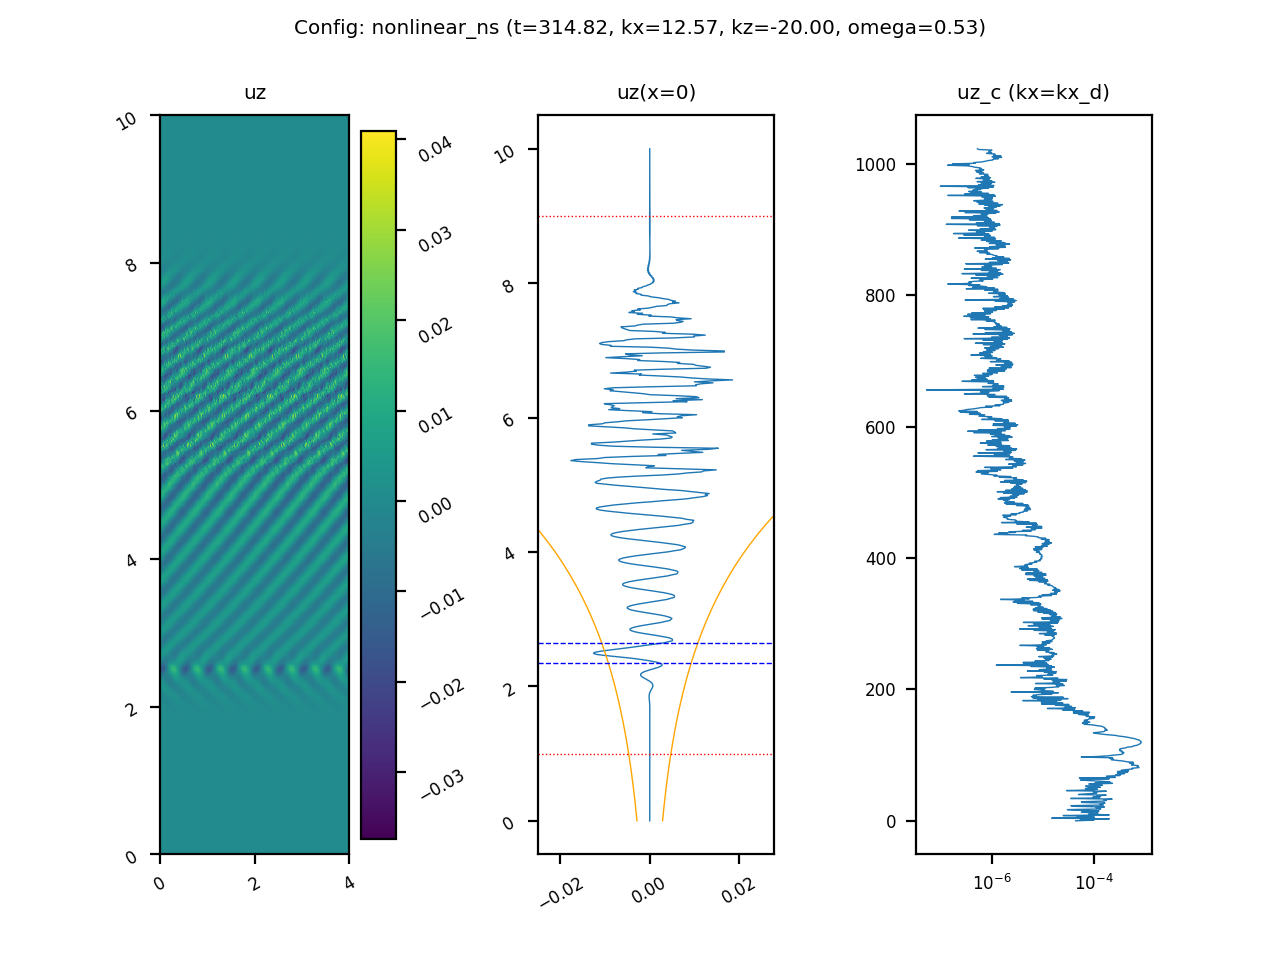
\includegraphics[width=\textwidth]{figs/nonlin_ns.png}
        \caption{Nonlinear simulation with Navier-Stokes regularization. The
        mismatch of the analytical envelope is again not significant. The
        supposed PSI from the non-regularized system is clearly just ringing
        from starting the forcing in discontinuous fashion.}
    \end{subfigure}\hfill
    \begin{subfigure}{0.47\textwidth}
        \centering
        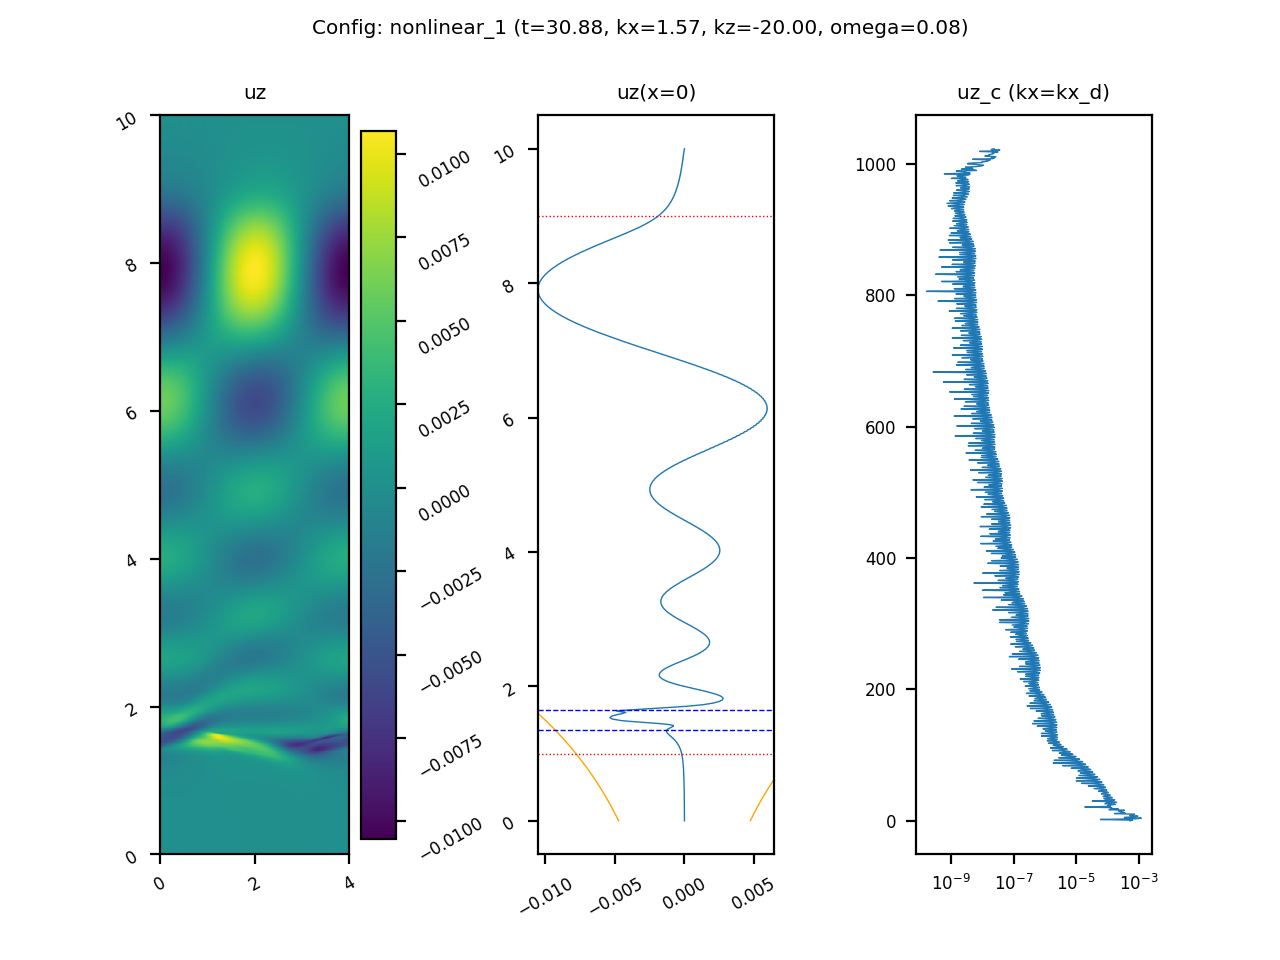
\includegraphics[width=\textwidth]{figs/nonlin_driving_blowup.png}
        \caption{Another consequence of starting the forcing in discontinuous
        fashion, nonlinear terms amplify the waveform in the driving zone and
        produces nonphysical shocks.}\label{fig:blowup}
    \end{subfigure}
    \caption{The four simulation snapshots above include the following notation:
        the left plot is a simple 2D plot of the $u_{1z}(x, z)$ field, the
        middle plot is a slice $u_{1z}(x=0, z)$ and the right plot plots the
        Chebyshev spectral expansion at the driving $k_x$. In the middle plots,
        the two dashed red lines indicate the damping zones, the dashed blue
        lines indicate the forcing zone $\pm 3\sigma$ and the orange solid lines
        indicate the analytically predicted envelope.}\label{fig:plots}
\end{figure}

\section{Future Work}

Mercifully omitted from this writeup are all of the misguided efforts that were
slowly revised out over time. Nevertheless, against all odds we find ourselves
very near conquering the 2D toy problem, with a few remaining difficulties to be
elaborated below.

\subsection{Remaining 2D Work}

We are very close to having a full working simulation of 2D wave breaking
without numerical singularities. The largest further obstacle that stands in our
way is computational expense, which is being rectified presently within the
group. Compounding our difficulties are that, in the $k_x \ll k_z$ limit that
most astrophysical IGWs find themselves in, the group velocity is extremely
slow, and so requiring resolving $N^{-1}$ timescales results in a very slow
simulation. Even so, we should soon understand where the dissipation in these
excited IGWs occurs as they break via nonlinear processes.

\subsection{3D Work}

\lstinline{Dedalus} has been adapted for 3D work, using spherical harmonics and
Chebyshev polynomials, so the software package is sufficiently up-to-date for
our problem. Nevertheless, 3D calculations will be even more expensive and will
likely carry with them another host of instabilities to sort out. Armed with our
understanding of these 2D difficulties, however, it should be much easier to
tackle.

We also intend to extend our 3D calculations to realstic WD equations of state
and density profiles\cite{fullerI}, such as those in \autoref{fig:eos}.
These will all have to be adapted somewhat to fit the requirements of
\lstinline{Dedalus}.
\begin{figure}[t]
    \centering
    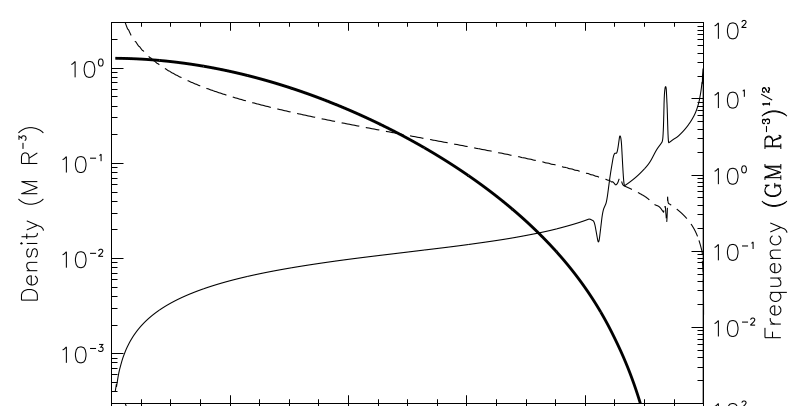
\includegraphics[width=\textwidth]{figs/fuller_eos.png}
    \caption{Dynamical variables for a realistic WD model. The thick line is the
    density and the thin line is $N^2$. The dashed line is the square of the
    Lamb frequency, not discussed in this paper but important to 3D
    waves.}\label{fig:eos}
\end{figure}.

\section{Conclusion and Acknowledgements}

In conclusion, we are very close to a numerical solution to the 2D plane
parallel atmosphere IGW breaking problem, with only a few more kinks to sort
out. With this, we should be able to interpret our results within the framework
of existing theory and, after having understood this thoroughly, generalize our
approach to the full realistic 3D problem.

I would like to thank Professor Dong Lai for advising me both as a lab member
and as a first year graduate student during the past year. I would also like to
thank Daniel Lecoanet for explaining his unending back of numerical tricks for
using \lstinline{Dedalus} to me.

\clearpage
\bibliographystyle{plainnat}
\renewcommand{\bibname}{References}
{\scriptsize \bibliography{q_writeup}}

\end{document}

